%%% -*- TeX-engine: xetex -*-
\documentclass{beamer}

% for themes, etc.
\usepackage{times}  % fonts are up to you
\usepackage{graphicx}
\usepackage{color}
\mode<presentation>
{
 \usetheme{Copenhagen}
 \usecolortheme{seahorse}
}
\usepackage{xeCJK}
\setCJKmainfont{WenQuanYi Micro Hei}

\title{基于翻译技术的流量调度}
\author{王文鑫}
\date{2016年1月5日}
\AtBeginSection[]
{
\begin{frame}<beamer> 
\frametitle{梗概}
\tableofcontents[currentsection]
\end{frame}
}

\begin{document}

\begin{frame}
\titlepage
\end{frame}

\section{背景介绍}
\subsection{MAP-T}

\begin{frame}
  \frametitle{MAP-T}
  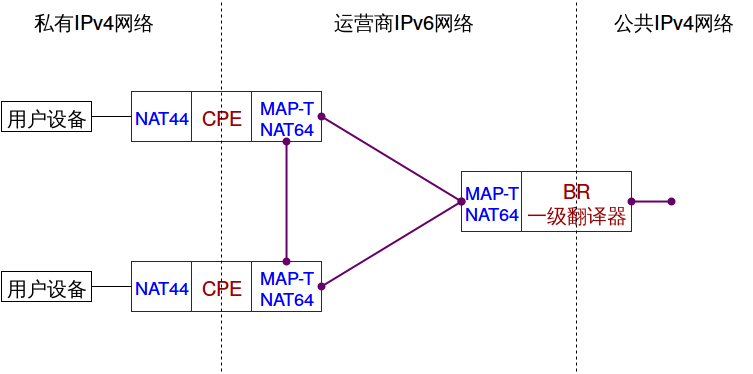
\includegraphics[width=\textwidth]{figs/MAP-T.png}  

  使用IPv6网络,将内部IPv4网络与公共IPv4网络相连
\end{frame}

\begin{frame}
  \frametitle{MAP}
\end{frame}

\begin{frame}
  \frametitle{MAP-T}
\end{frame}

\begin{frame}
  \frametitle{Cookie Approach}

  Now, suppose we have only 4/5 of a cookie.

  Then we can feed only 4/5 as many people, i.e.

  $$
  \frac{4}{5} \times \frac{3}{2} ~ people
  $$

  \pause 

  So we've derived the ``invert and multiply'' rule in the general case:

  $$
  \frac{4}{5} \div \frac{2}{3} = \frac{4}{5} \times \frac{3}{2}
  $$ 

\end{frame}

\section{A Geometry Proof}

\begin{frame}
  \frametitle{A Geometry Proof}

  (Illustrating {\sc beamer}'s $\backslash$uncover command.)
  \vskip 0.5in

  \begin{theorem}
    The angles in a triangle sum to $180^{\circ}$.
  \end{theorem}

  \pause

  Plan:  Extend AC past C to D.  Draw CE parallel to AB.

\end{frame}

\begin{frame}

  \begin{proof}

    \begin{tabular}{ll}
      % uncover makes advanced overlay
      \uncover<1->{1. u = y} & \uncover<2->{Alternate angles of a
                               transveral.} \\ 
      \uncover<3->{2. v = x} & \uncover<4->{Consecutive interior angles of a
                               transveral} \\ 
      \uncover<5->{3. z+u+v = $180^{\circ}$} & \uncover<6->{ACD is a straight
                                               line.} \\ 
      \uncover<7->{4. z+y+x = $180^{\circ}$} & \uncover<8->{Substitution
                                               from Steps 1 and 2.} \\
    \end{tabular}

  \end{proof}

\end{frame}

\section{More Advanced Features of {\sc beamer}}

\begin{frame}
  \frametitle{More Advanced Features of {\sc beamer}} 

  \begin{itemize}

  \item This tour just scratches the surface.  
    \pause

  \item {\sc beamer} has enough features to fill a 210-page user manual!  
    \pause

  \item Advanced example:
    \url{http://latex-beamer.sourceforge.net/beamerexample1.pdf}.

  \end{itemize}

\end{frame}

\end{document}
